% !TeX root = paper.tex


\chapter{車両タイプ判別モデルについて}
%\section{この章で書くこと}
%\begin{itemize}
%	\item 学習の実行
%	\item 性能評価
%	\item 作成したモデルの使い方
%	\item 出力されるものについて
%\end{itemize}


\section{学習の実行}
作成したデータセットとYOLOv8を用いてモデルの学習を行い,分類用と識別用の2種類のモデルを作成した.
分類モデルでは静止画での判別しかできない.動画から車両タイプを判別するために識別モデルを作成した.


\section{作成したモデルの使い方}
識別モデルと分類モデルで使い方はほぼ同じである.
作成したモデルをロードして,モデルに画像または動画を渡すと識別または分類をすることができる.\\
識別
\begin{verbatimx}
	from ultralytics import YOLO
	model = YOLO("作成した識別モデルのパス")
	results = model.predict("画像または動画のパス")
\end{verbatimx}

分類
\begin{verbatimx}
	from ultralytics import YOLO
	model = YOLO("作成した分類モデルのパス")
	results = model("画像のパス")
\end{verbatimx}

\section{出力されるもの}
17種類の車両が各10枚ずつ,合計170枚のテストデータセットを識別した際にターミナルに出力されるものを図 \ref{output}に示す.
左端のimageから,「何枚目か」「画像のパス」「入力画像のサイズ」「予想クラス番号」「予想クラス番号に対応する車両タイプ」「識別にかかった時間」が画像ごとに出力される.
識別時にsave = Trueを追加すると入力画像に識別結果が追記された画像が出力される.
識別時にsave\_txt = Trueを追加すると画像ごとに予想クラスと座標情報がテキストファイルで出力される.
モデルを動かした際に端末に出力されるものを図\ref{output}に記す.
\begin{figure}	
	\centering
	\includegraphics[width=\linewidth]{fig/a.pdf}
	\caption{端末に出力されるもの}\label{output}
\end{figure}

\section{作成したモデルの評価と考察}

\subsection{分類モデルの評価}
%分類モデルの評価を図\ref{CLS}に示す
\begin{figure}	
	\centering
	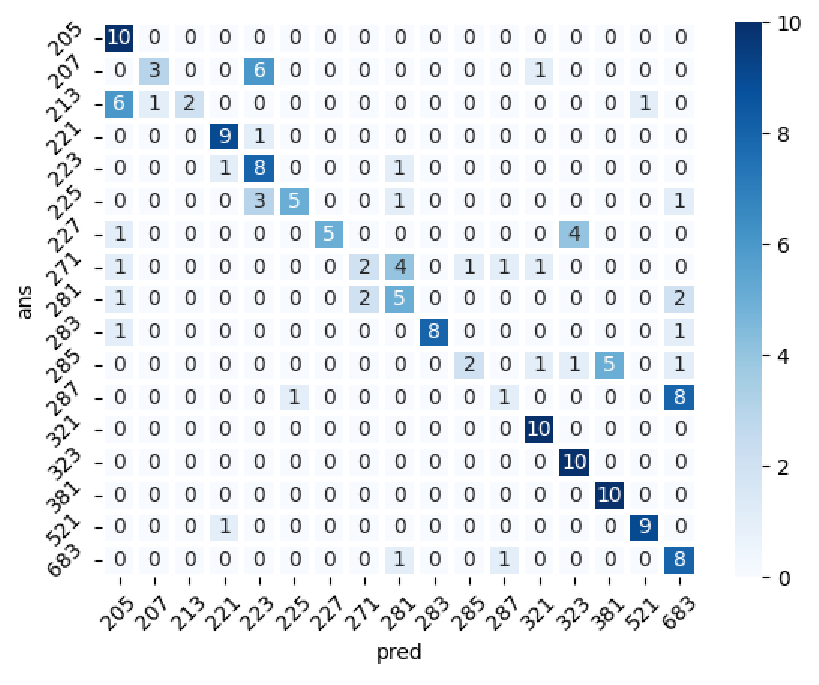
\includegraphics[width=\linewidth]{chap4/fig/classify_results.pdf}
	\caption{分類モデルの混合行列}
	\label{CLS}
\end{figure}
作成した分類モデルを用いてテストデータセットの分類を行った結果をを図\ref{CLS}に示す.
縦軸が予測した車両タイプ,横軸が正解の車両タイプとするグラフである.


\subsection{識別モデルの評価}
識別時には,どの車両タイプにも当てはまらないと識別されることがある.その場合の車両タイプは0として識別モデルの混合行列を作成した.
識別結果を表\ref{fig:chartdet} に示す.\\
%NaNとは識別成功数または識別失敗数が0のときに,IoUの平均が出せない場合の値である.\\
% TODO: \usepackage{graphicx} required
\begin{figure}[H]
	\centering
	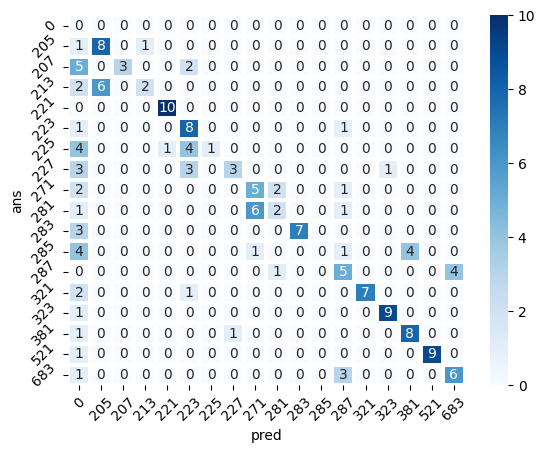
\includegraphics[width=\linewidth]{chap4/fig/predicted_results.jpg}
	\caption{識別モデルの混合行列}
	\label{fig:chartdet}
\end{figure}



\subsection{考察}
正解率は車両タイプによって異なることがわかる.287系と683系のように外見が似ている電車だと,誤判別していることが多かった.
287系を図\ref{fig:287},683系を図\ref{fig:683}に示す.
%データセットの画質を落とすと誤判別が増えた.特に誤分類が多かった三種類の電車の画質を上げても結果はあまり変わらなかった.
%限られたストレージでは,データセットの画質を変化させて判別結果を向上させることは難しいと考えられる.SSDの容量に制限がない場合,大量の高画質のデータでデータセットを作成することで判別結果が改善される可能性があると考えられる.
%各車両タイプの画像の枚数に差があったことが判別結果に影響を与えていると考えられる.
データセットの画像の枚数が少ない車両タイプの判別結果が必ず悪くはならなかった.
画像の枚数が判別結果に影響を与えるのではなく,車体の特徴が鮮明に写っている画像の枚数が判別結果に影響を与えると考えられる.
判別精度の向上のために,データセットとして質の悪い画像を大量に集めるのではなく,車体の特徴が鮮明に写っている画像を車両タイプごとに集める必要があったと考えられる.

同じ画像を使って,分類用と識別用の2種類のデータセットを作成した.分類モデルの混合行列と識別モデルの混合行列が似ているため,車両タイプを知るためのシステムを作る際には,識別モデルのみを作成することで画像と動画の両方に対応した車両判別システムを作成でき,電車の車両タイプを知ることができるようになると考える.

% TODO: \usepackage{graphicx} required
\begin{figure}
	\centering
	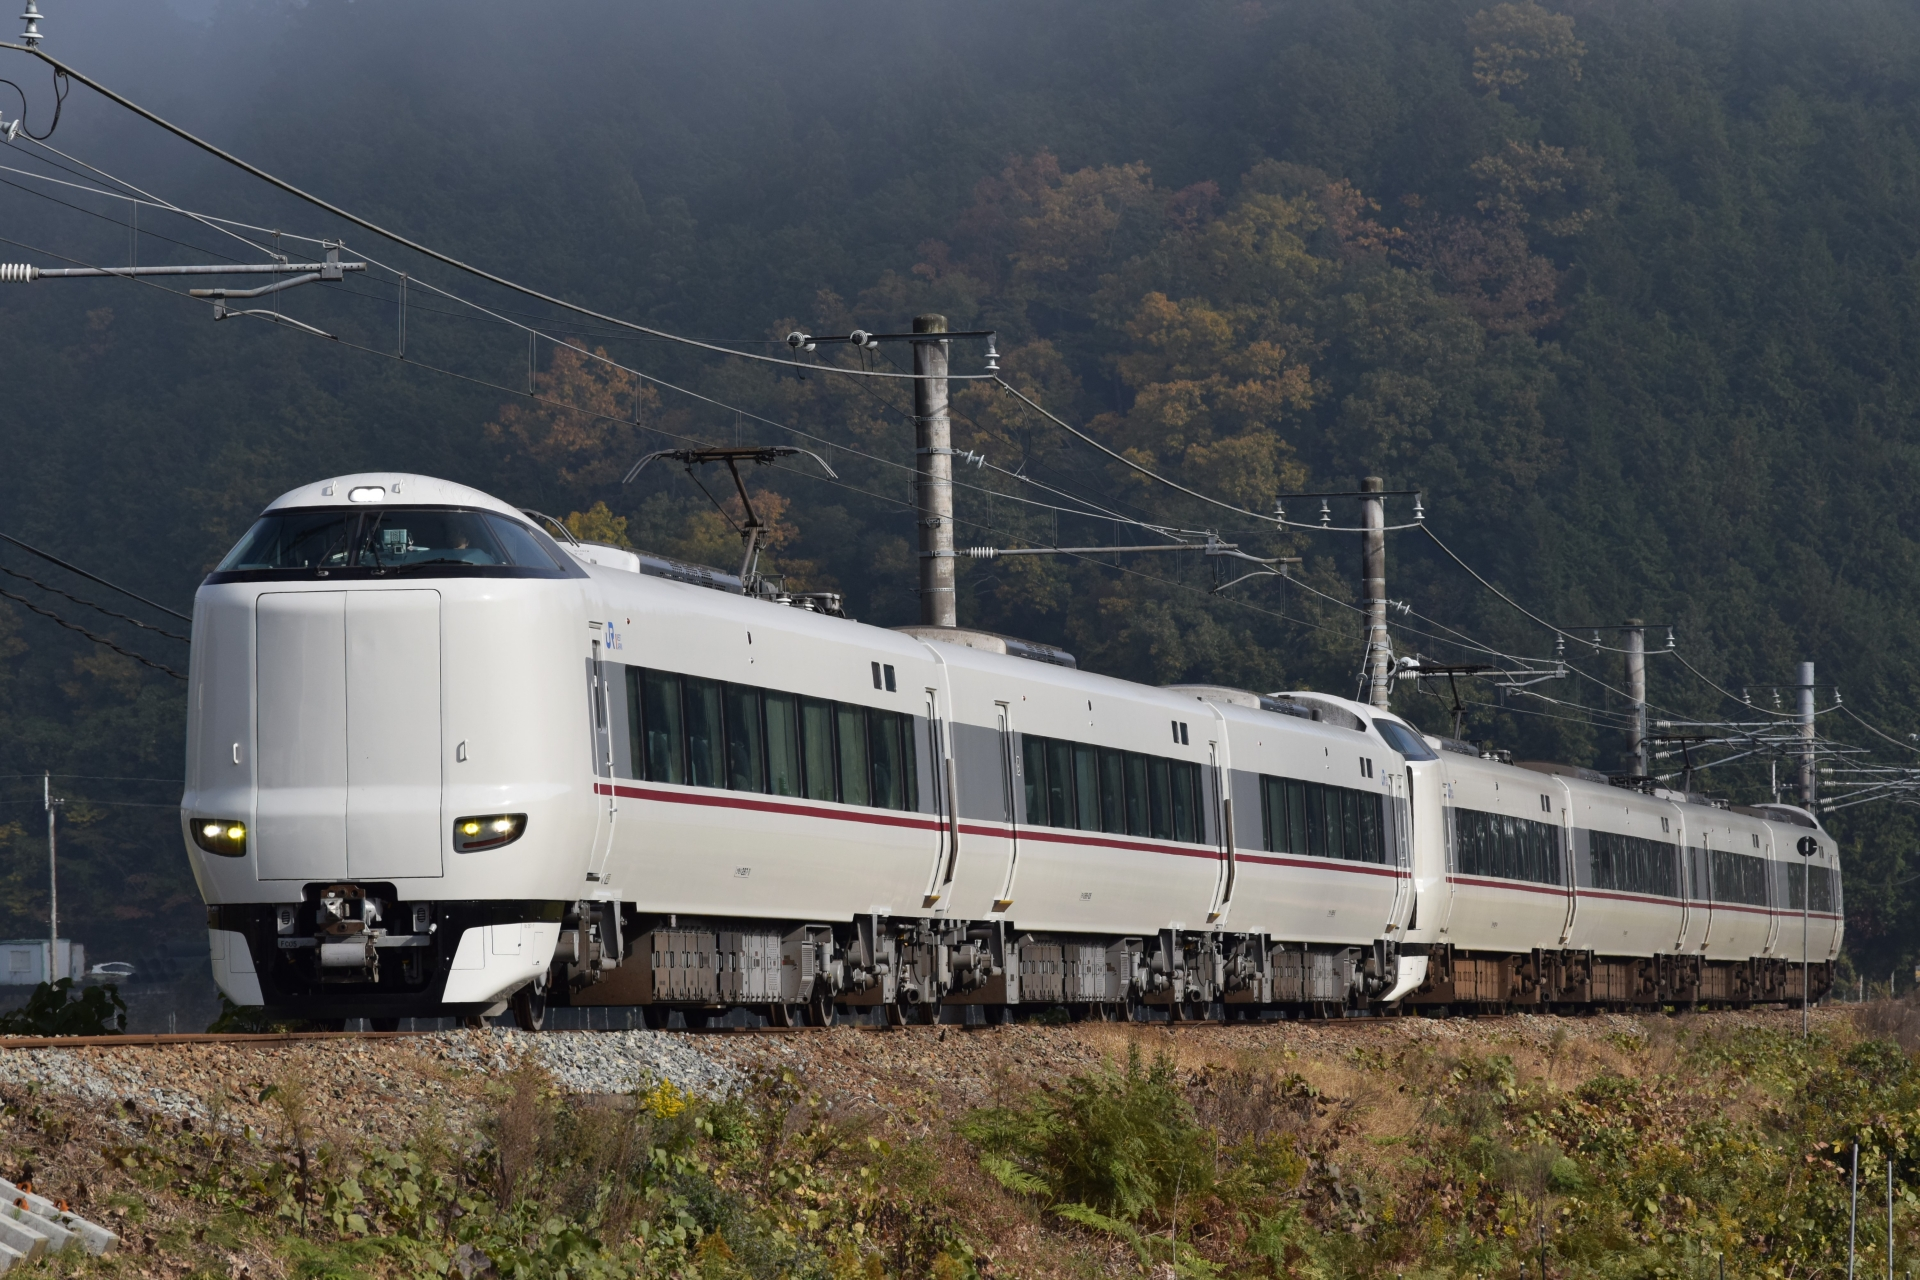
\includegraphics[width=0.7\linewidth]{chap4/fig/287}
	\caption{287系}
	\label{fig:287}
\end{figure}

% TODO: \usepackage{graphicx} required
\begin{figure}
	\centering
	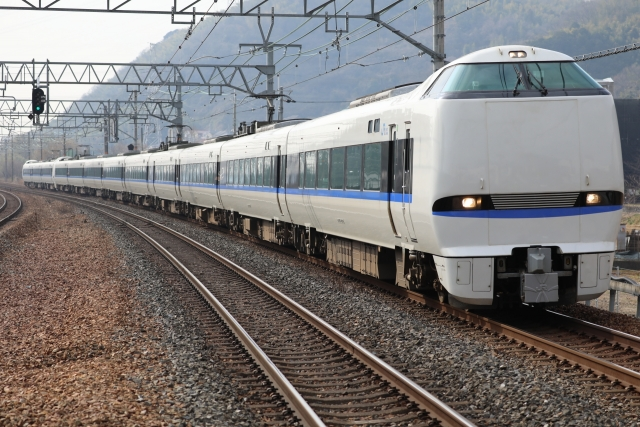
\includegraphics[width=0.7\linewidth]{chap4/fig/683}
	\caption{683系}
	\label{fig:683}
\end{figure}

